%----------------------------------------------------

\begin{frame}
  \frametitle{Parallélisation de Routino}
  \framesubtitle{Deux approches possibles}
  \begin{itemize}
  \item Parallélisation de l'algorithme :
    \begin{itemize}
    \item Trop de dépendances de données
    \item Trop de points de synchronisation
    \end{itemize}
    \vspace{1em}
  \item Parallélisation par segments
    \begin{itemize}
    \item Prédécouper l'itinéraire en segments
    \item Calculer chaque segment séparément
    \end{itemize}
  \end{itemize}
\end{frame}

% --------------------------------------------------

\begin{frame}
  \frametitle{Parallélisation de Routino}
  \framesubtitle{Approche par segments}
  \begin{columns}[t]
    \visible<1->{
      \begin{column}{0.5\textwidth}
        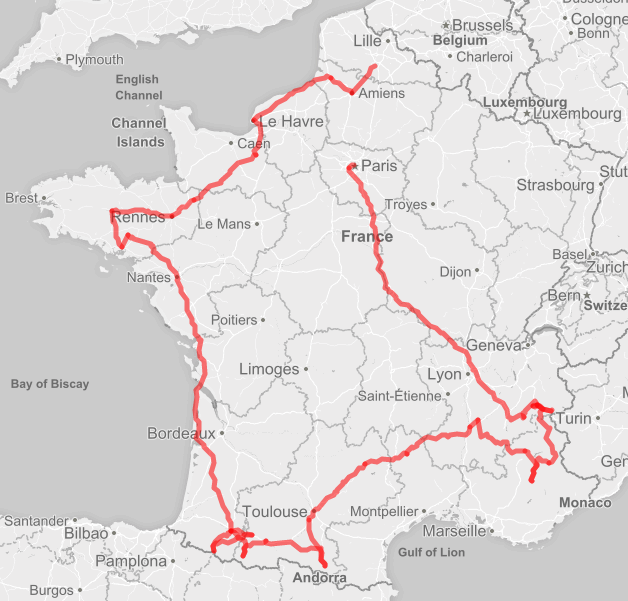
\includegraphics[scale=0.25]{include/tourfrance_mono.png}
      \end{column}
    }
    \visible<2->{
      \begin{column}{0.5\textwidth}
        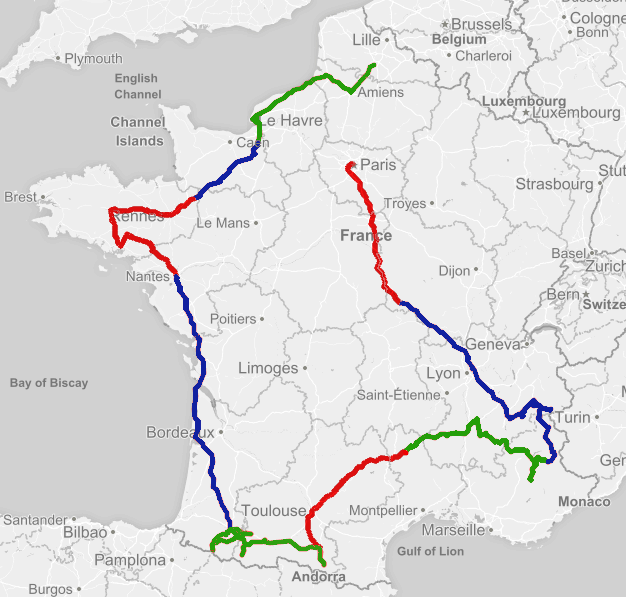
\includegraphics[scale=0.25]{include/tourfrance_multi.png}
      \end{column}
    }
  \end{columns}
  \visible<3->{
    \begin{alertblock}{Difficulté d'implantation}
      Les segments doivent être indépendants et le nombre de points de
      synchronisation faible.
    \end{alertblock}
  }
\end{frame}

% --------------------------------------------------

\begin{frame}
  \frametitle{Parallélisation de Routino}
  \framesubtitle{Déroulement de l'exécution}
  \begin{center}
    \only<1>{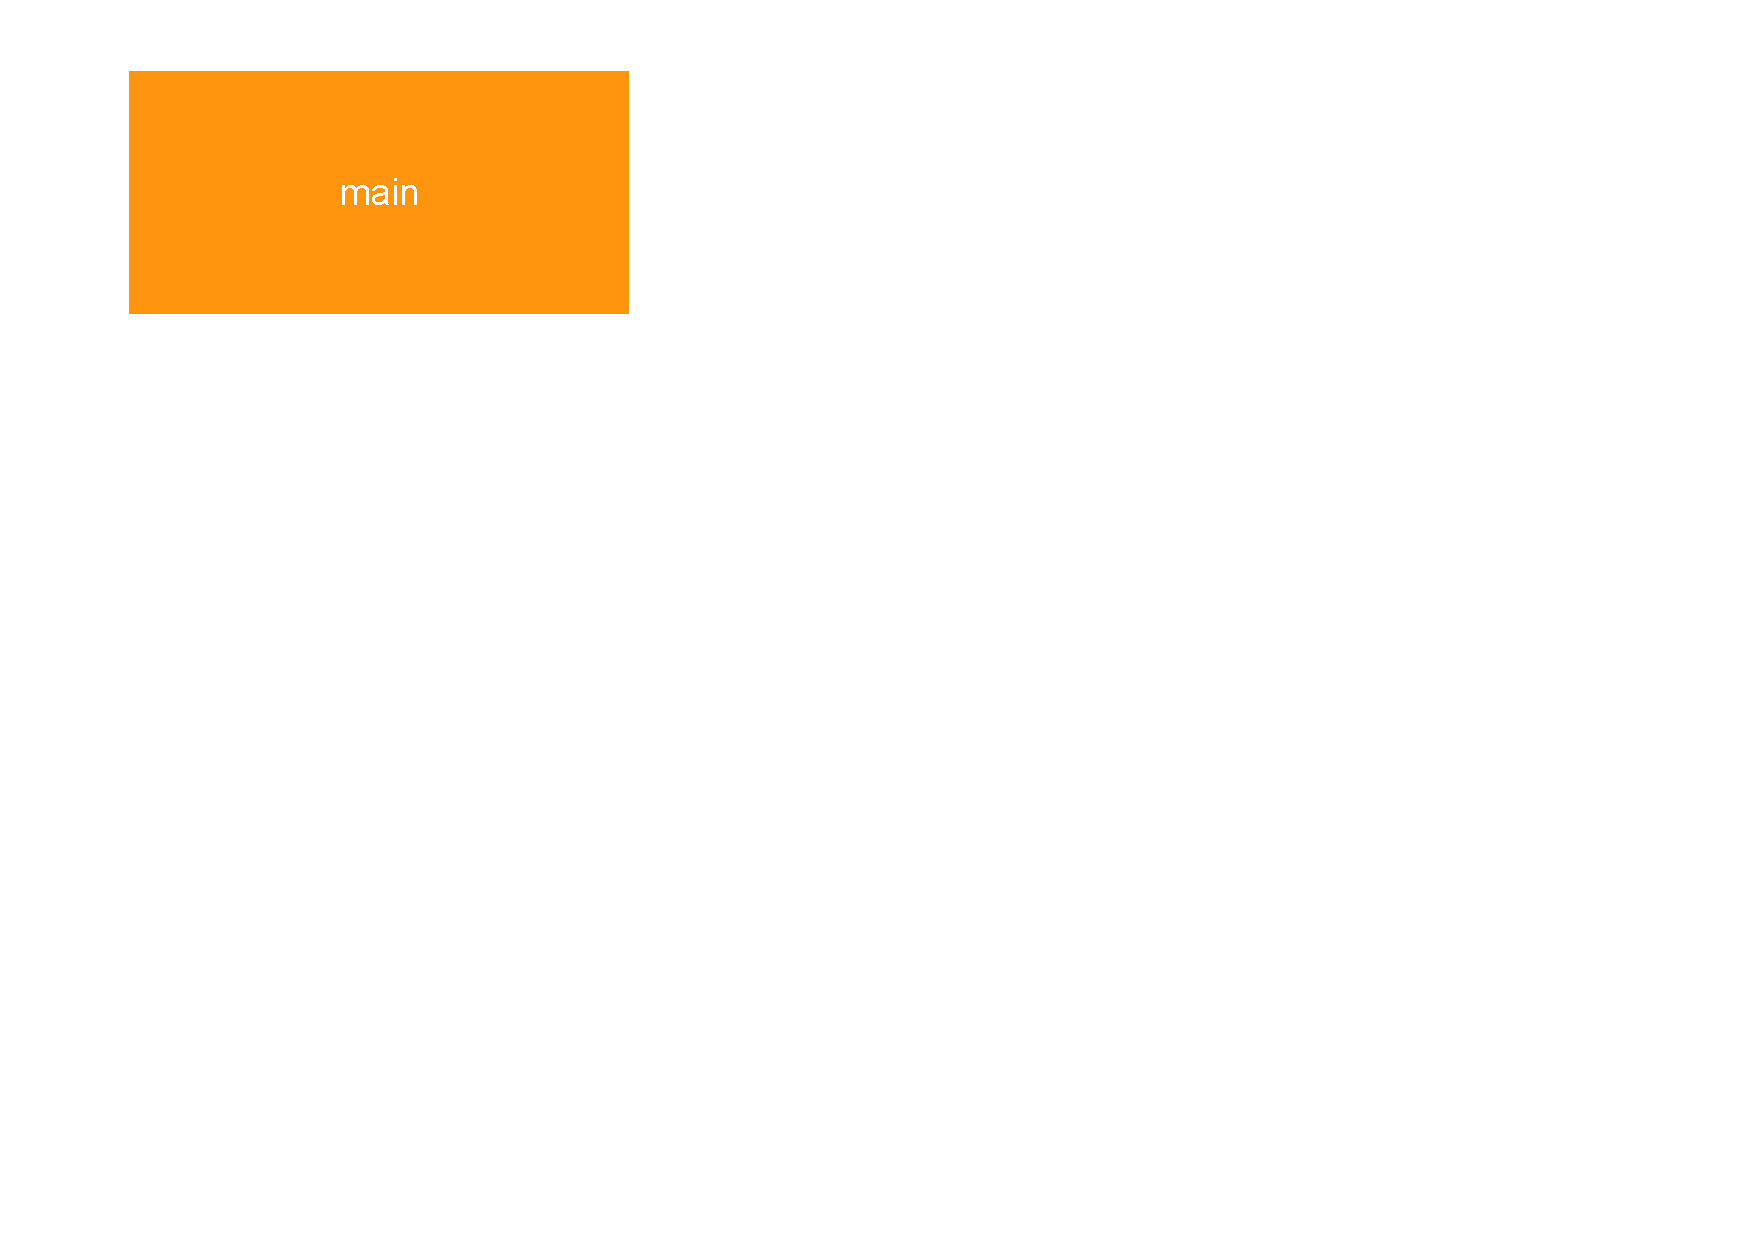
\includegraphics[scale=0.34]{include/multi1.pdf}}
    \only<2>{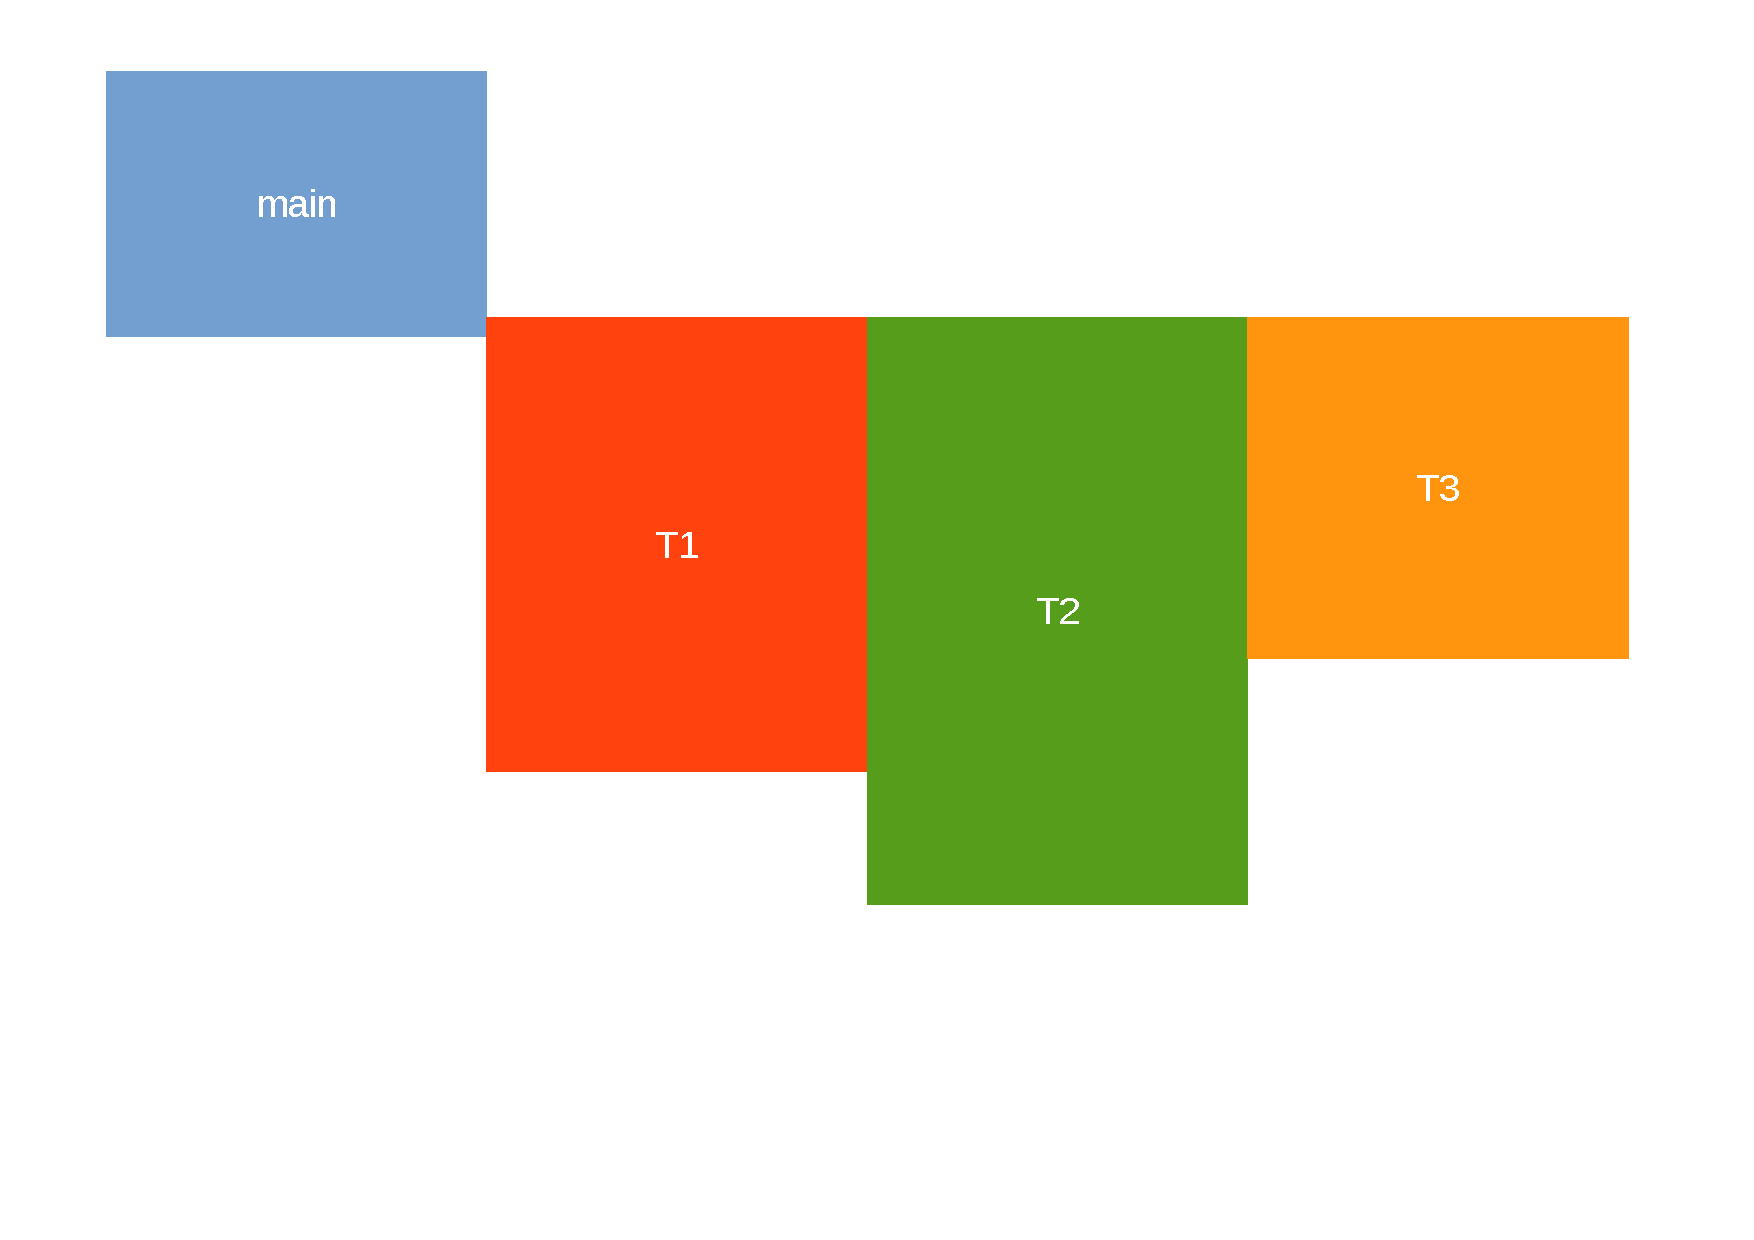
\includegraphics[scale=0.34]{include/multi2.pdf}}
    \only<3>{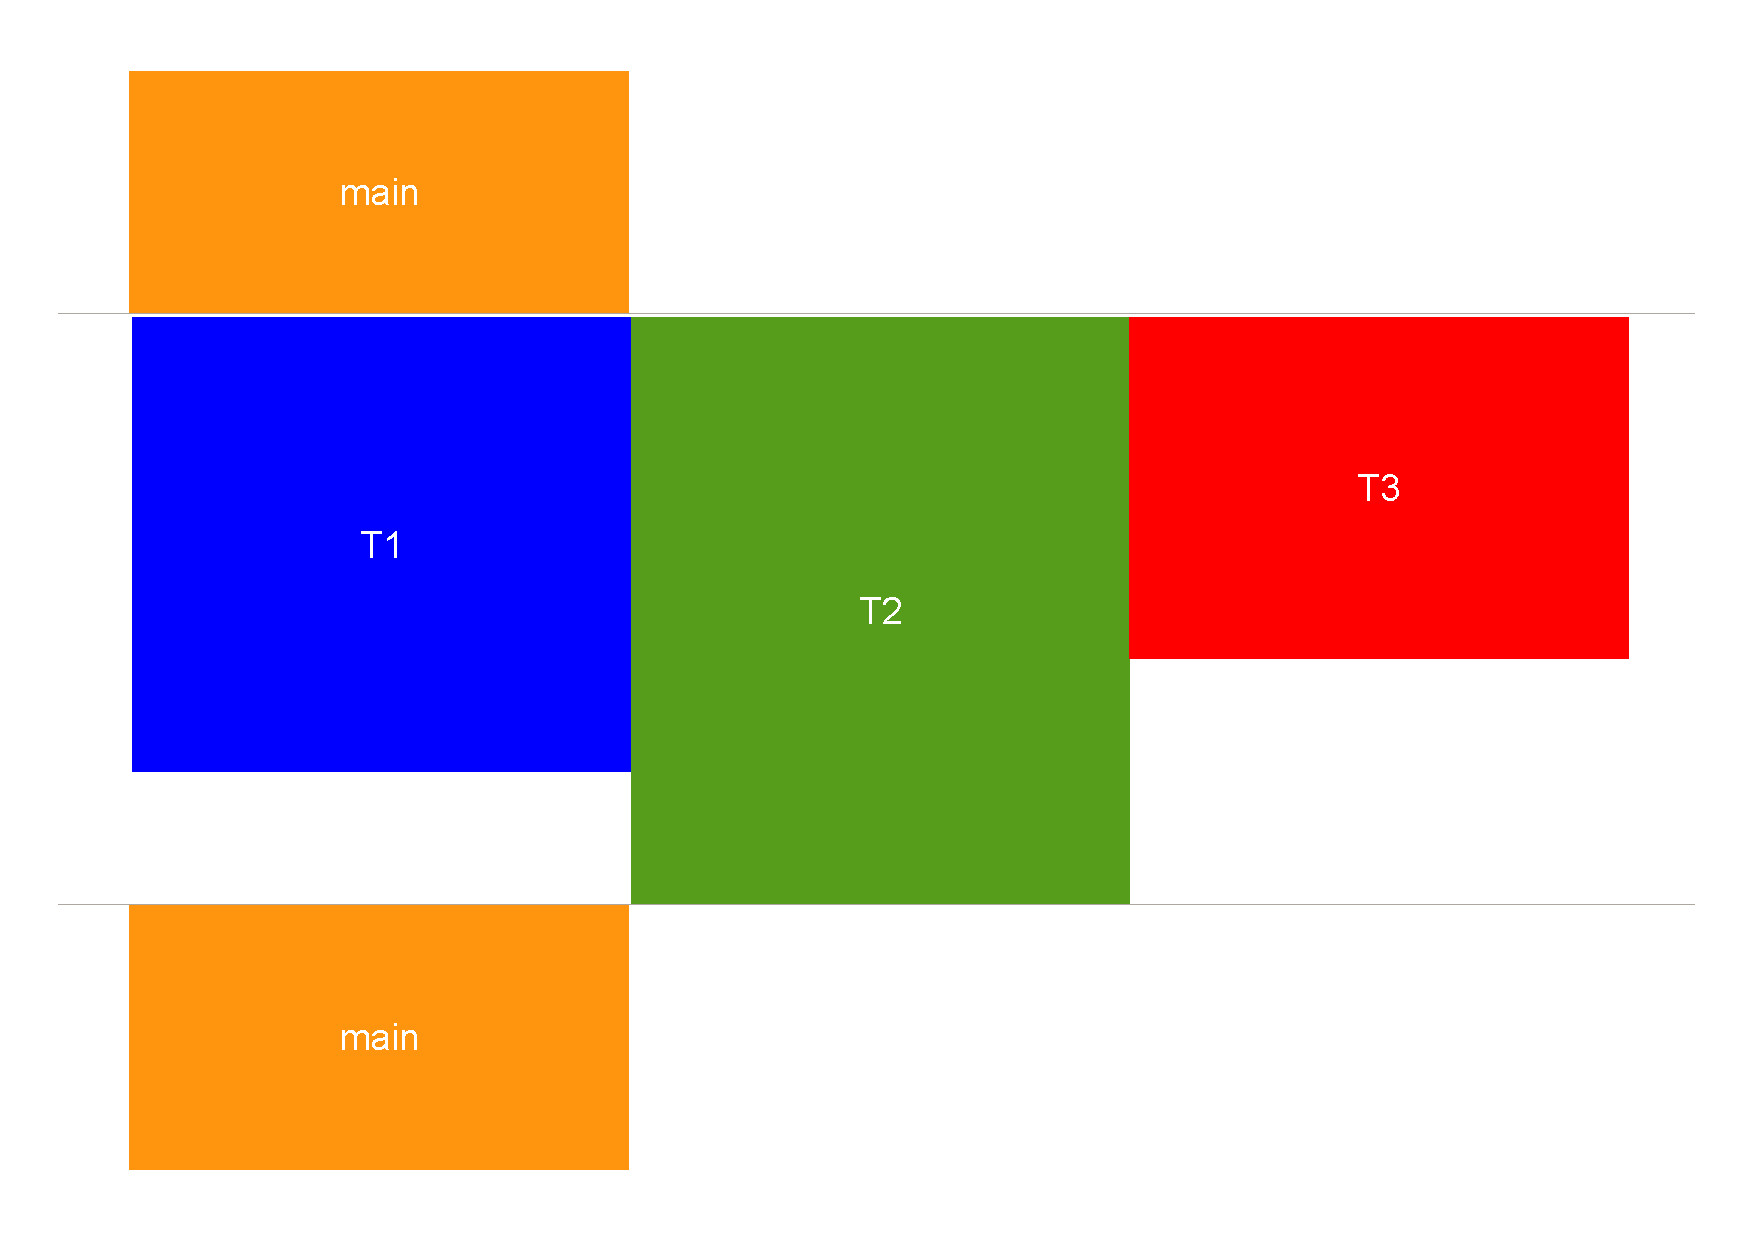
\includegraphics[scale=0.34]{include/multi3.pdf}}
  \end{center}

\end{frame}

% --------------------------------------------------

\begin{frame}
  \frametitle{Parallélisation de Routino}
  \framesubtitle{\'Evaluation - Utilisation CPU par tâche}
  
  \begin{center}
    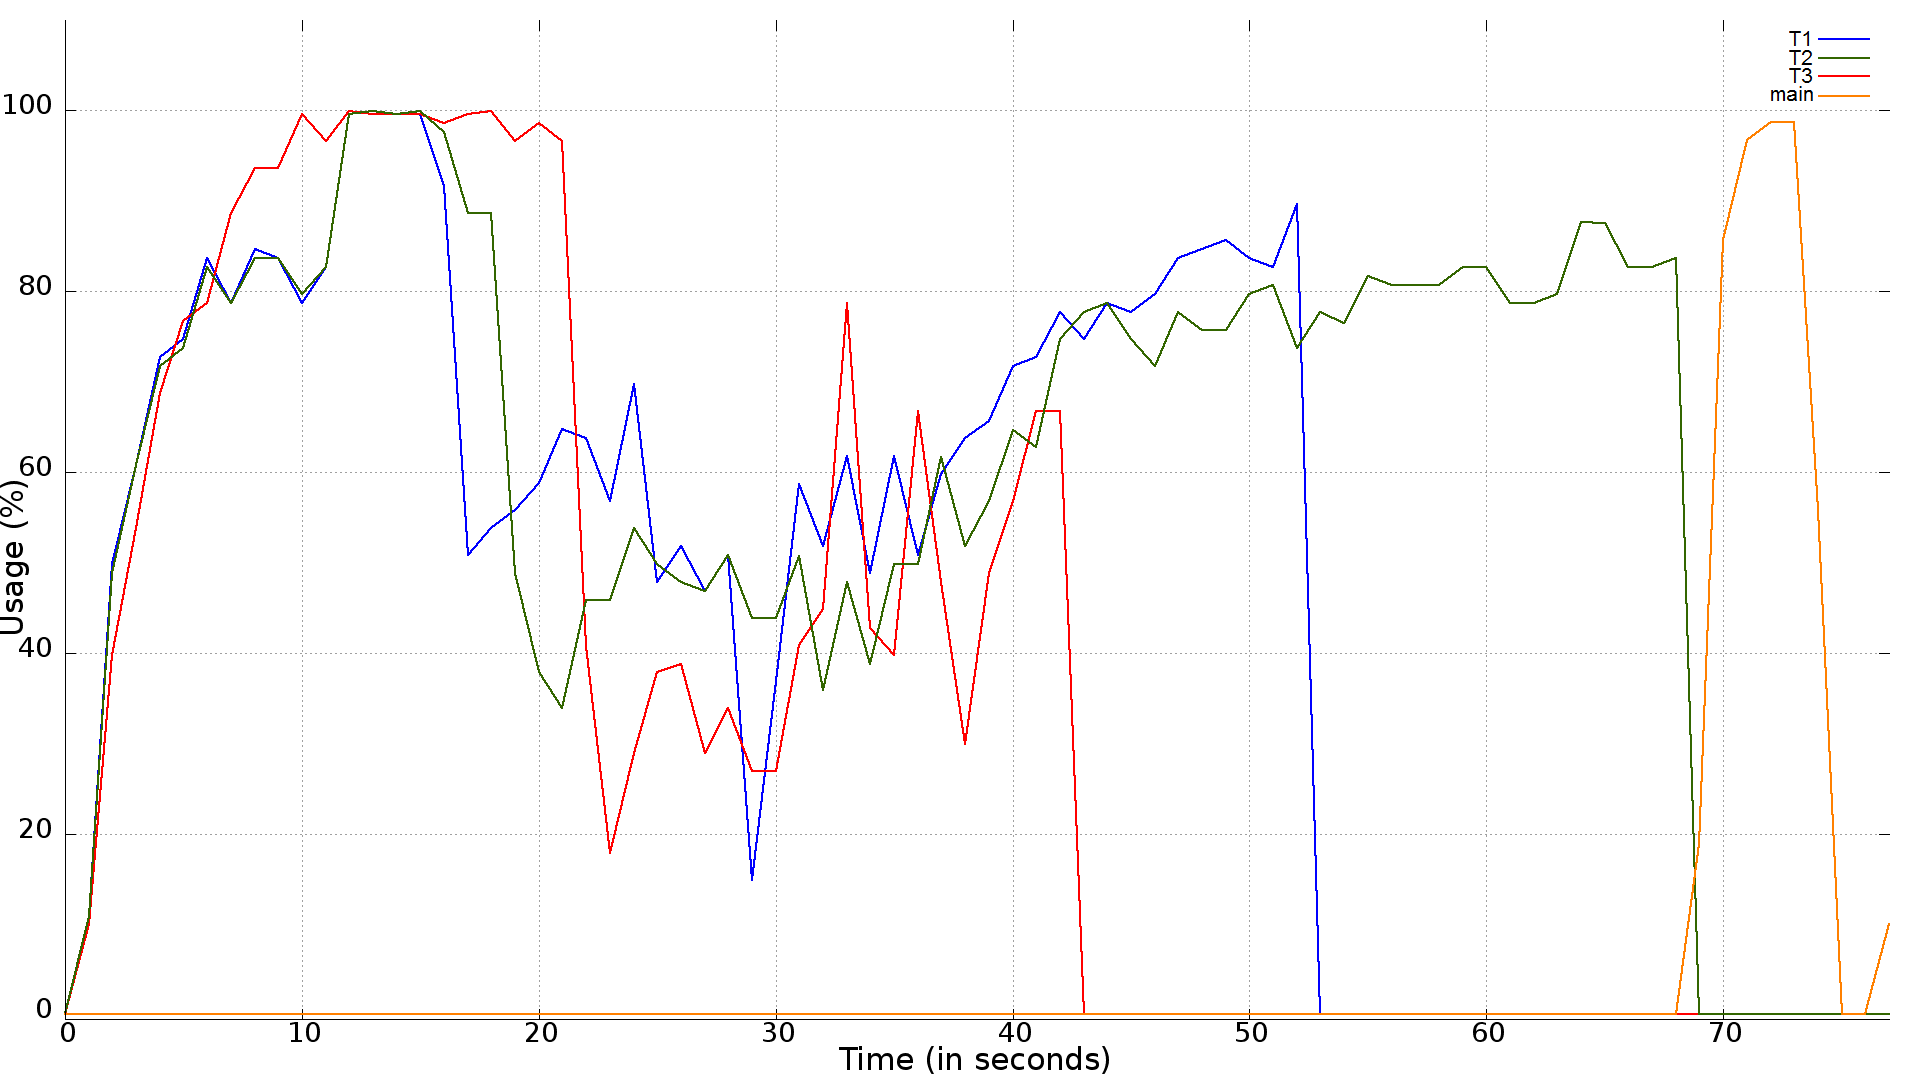
\includegraphics[scale=0.18]{include/thread_usage.png}
  \end{center}
  \visible<2>{
    \begin{exampleblock}{Observations}
      On note les terminaisons différées des tâches et la reprise du
      \texttt{main} après la barrière de synchronisation.
    \end{exampleblock}
  }
\end{frame}

% --------------------------------------------------

\begin{frame}
  \frametitle{Parallélisation de Routino}
  \framesubtitle{\'Evaluation - Gain de performance}

  \begin{center}
    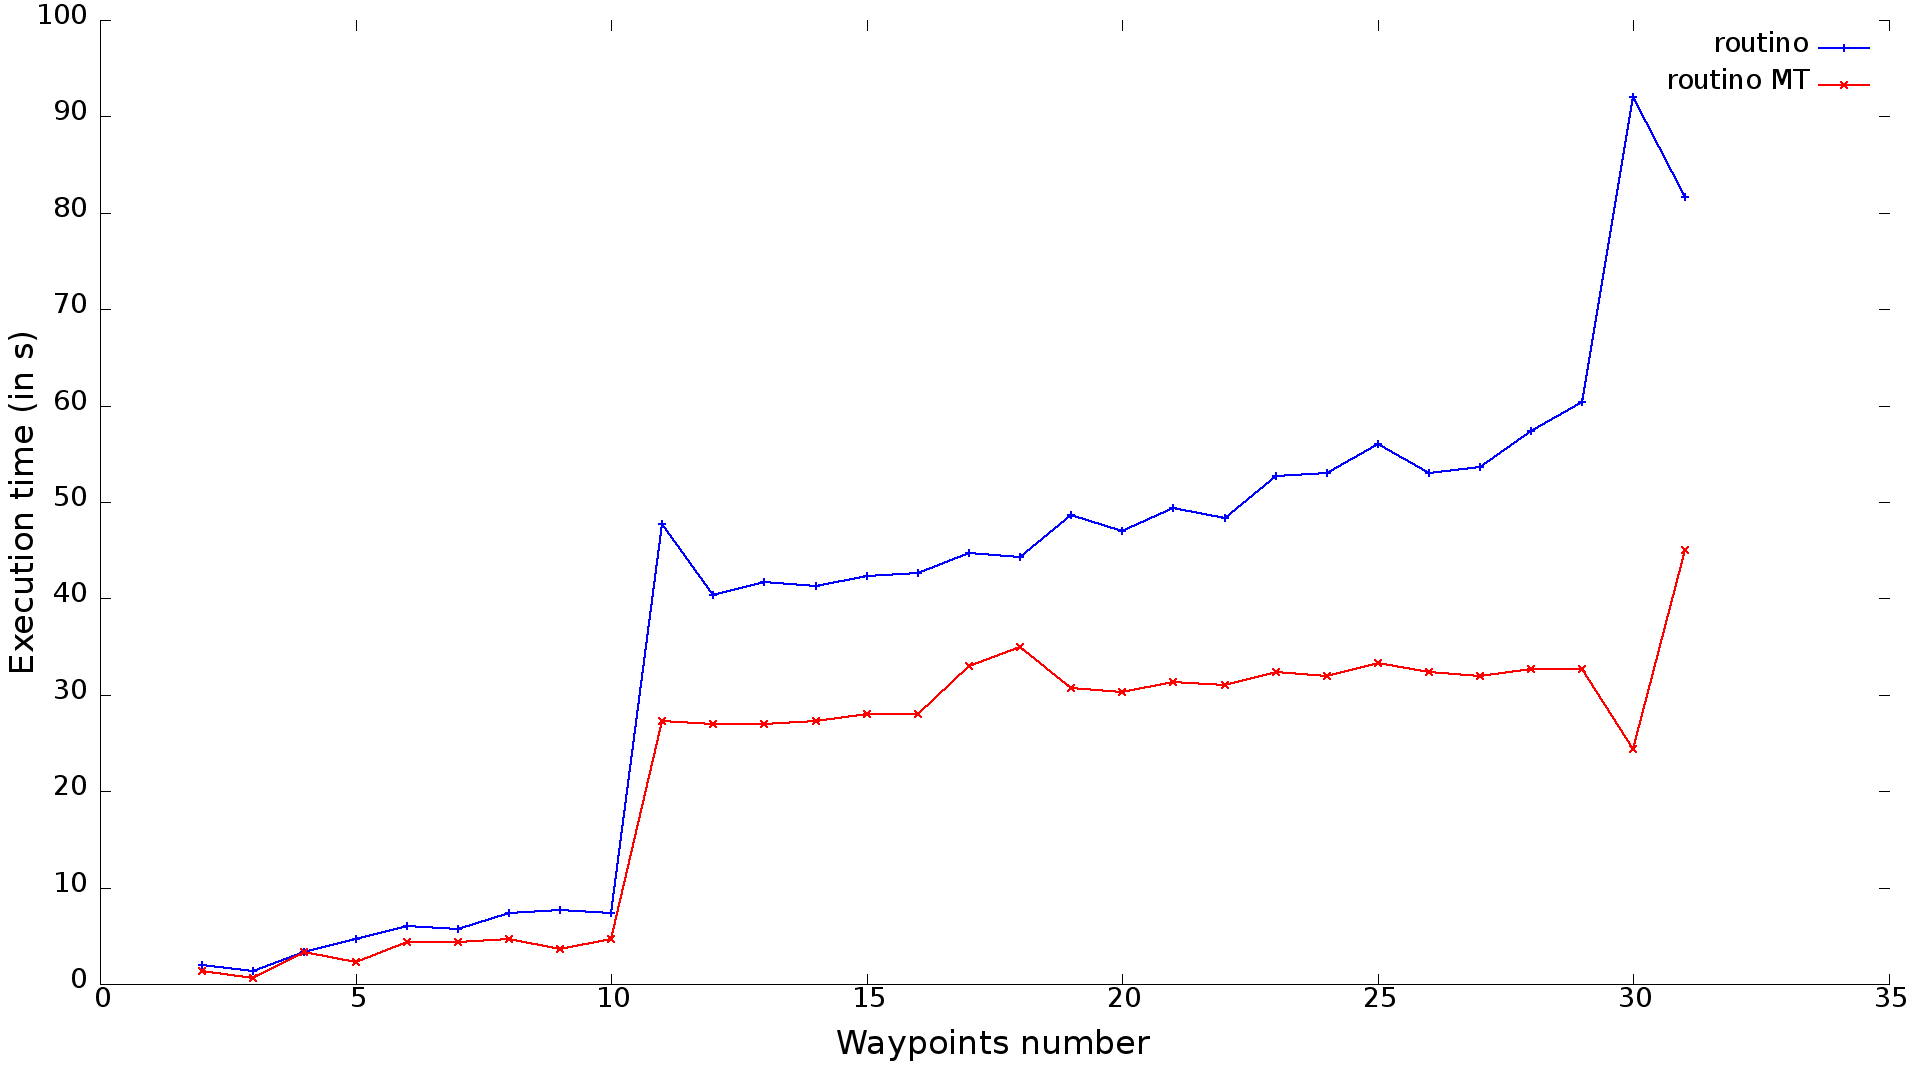
\includegraphics[scale=0.18]{include/speedup.png}
  \end{center}
  \visible<2>{
    \begin{exampleblock}{Observations}
      \begin{itemize}
        \item Temps divisé par 2 au mieux car plus de calculs par segment
        \item Les longs segments offrent un meilleur gain
      \end{itemize}
    \end{exampleblock}
  }
\end{frame}
